\documentclass[14pt,a4paper]{extarticle}
\newcommand{\judul}{Pendalaman Materi UTS SMA 68}
\newcommand{\penulis}{bintangpelajar.com}
\usepackage[latin1]{inputenc}
\usepackage{longtable}\usepackage{amsmath}
\usepackage{microtype}
\usepackage[none]{hyphenat}
\usepackage{verbatim}
\usepackage{amsfonts}
\usepackage{amssymb}
\usepackage{enumitem}
\renewcommand{\familydefault}{\sfdefault}
\usepackage{mathpazo}
\renewcommand{\rmdefault}{put}
\usepackage{enumitem}
\usepackage[dvipsnames,svgnames]{xcolor}
\usepackage{tkz-euclide}
\usetkzobj{all}
\usepackage{graphicx}
\usepackage{fancyhdr}
\usepackage{tikz} 
\usetikzlibrary{quotes,angles}
\usepackage{adjustbox}
\usepackage{multicol}
\usepackage{lipsum}
\usepackage[headsep=0.2cm,footskip=2pt,top=1.2cm,bottom=1cm,left=1cm,right=1cm]{geometry}
\usepackage{cancel} \usepackage{xcolor}
\usepackage{tcolorbox}
\usetikzlibrary{decorations.pathmorphing,patterns}
\usetikzlibrary{decorations.pathreplacing,calc}
 \newcommand\coret[2][red]{\renewcommand\CancelColor{\color{#1}}\cancel{#2}}
\SetLabelAlign{Center}{\hfil\makebox[1.0em]{#1}\hfil}

\newtcolorbox{mybox}[1][] { colframe = blue!10, colback = blue!3,boxsep=0pt,left=0.2em, coltitle = blue!20!black, title = \textbf{jawab}, #1, } 

%---------- kunci (jika 1 ) muncul
\def\tampilkunci{0}
\newcommand{\hide}[1]{\ifnum\tampilkunci=1
%
\begin{mybox}
 #1
\end{mybox}
%
\vspace{\baselineskip}\fi}

\newcommand*\kunci[1]{\ifnum\tampilkunci=1
%
\tikz[baseline=(char.base)]{\node[red, shape=circle,draw,inner sep=0.5pt,xshift=2pt](char){#1};}\stepcounter{enumii}
\fi\ifnum\tampilkunci=0
%
\hspace{3pt}#1\stepcounter{enumii}
%
\fi}

%------------- MULAI FUNGSIKU ------------
\newcommand{\cartesius}[3]{
\draw[help lines] (-1,-1) grid (#1);
\foreach \x in {1,2,...,#2}{
\node at (\x,0)[scale=0.5]{\x};}
\foreach \y in {1,2,...,#3}{
\node at (0,\y) [scale=0.5]{\y};}}

\newcommand{\pers}[1]{\begin{align*} #1 \end{align*}}
% \sci{ }  misal  x 10^2  tinggal tulis 
% \sci{2} 
\newcommand{\sci}[1]{$\times 10^{#1}$}

\newcommand{\scip}[1]{\times 10^{#1}}

%----membuat tanda silang di samping text
\newcommand*\silang[1]{\tikz[baseline=(char.base)]{
\draw[red,thick](-0.2,-0.20)--(0.2,0.2);
\draw[red,thick](-0.2,0.20)--(0.2,-0.2);
\node[black](char){#1};
}}
%----- membuat tanda centang di mana saja
\newcommand*\centang[1]{\tikz[baseline=(char.base)]{
\draw[red, very thick](-0.2,0.1)--(-0.1,0)--(0.2,0.3);
\node(char){#1};
}}
%------------mewarnai text merah
\newcommand*\merah[1]{
\textcolor{red}{#1}}
\newcommand*\pilgan[1]{
\begin{enumerate}[label=\Alph*., itemsep=0pt,topsep=0pt,leftmargin=*,align=Center] #1 
\end{enumerate}}

%---- membuat pernyataan pada soal SBMPTN
\newcommand*\pernyataan[1]{
\begin{enumerate}[label=(\arabic*), itemsep=0pt,topsep=0pt,leftmargin=*] #1 
\end{enumerate}}

%------ lebar baris pada tabular
\newcommand{\baris}[1]{\renewcommand\arraystretch{#1} }
%\newcommand{\tabel}[2j]{\begin{tabular}{#1}
%\end{tabular}
%------------ END OF FUNGSIKU ----------- 





%--------------- begin{document}-----------
\pagestyle{fancy}
\fancyhf{} 
\rhead{\penulis}
\lhead{\judul}
\rfoot{Hal \thepage}
\begin{document}
\begin{center}
\begin{longtable}{|l|p{8cm}|p{9cm}|}
\hline 
1 &
Tiga buah partikel dengan massa $m$, $2m$, dan $3m$ dipasang seperti gambar.

\begin{tikzpicture}[scale=0.8]
\draw[<->](-3,0)--(3,0);
\draw[<->](0,2)--(0,-0.5);
\draw [fill=black](-1,0) circle (0.1cm) node [above,scale=0.7]{3m};
\draw[fill=black] (0,1) circle (0.1cm) node [right,scale=0.7]{2m};
\draw [fill=black](2,0) circle (0.1cm) node [above,scale=0.7]{m};
\node at (-0.5,0.2)[scale=0.7]{$a$};
\node at (0.1,0.5)[scale=0.7]{$a$};
\node at (1,0.2)[scale=0.7]{$2a$};
\end{tikzpicture}

Tentukan momen inersia sistem jika diputar terhadap sumbu $y$!
 &  \\ \hline
2 &
Suatu papan dengan panjang 1m. Momen gaya resultan terhadap poros pada gambar di bawah ini adalah . . . 

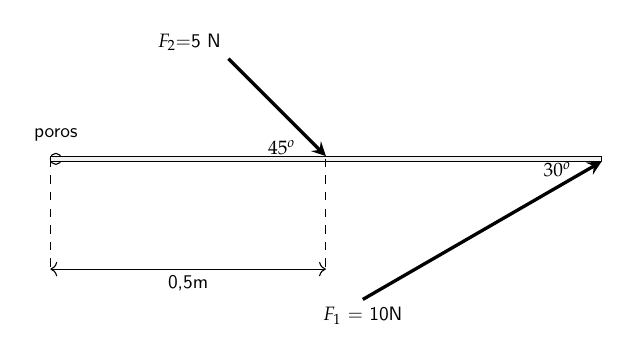
\begin{tikzpicture}[scale=0.7]
\draw (0.1,0) circle (0.1cm) node [above,scale=0.7,yshift=0.2cm]{poros};
\draw [fill=gray!10](0,0.05) rectangle (10,-0.05);
\draw [stealth-, very thick](5,0.05)--++(135:2.5)node [above left, scale=0.7]{$F_2$=5 N};
\draw [stealth-, very thick](10,-0.05)--++(210:5) node [below, scale=0.7]{$F_1$ = 10N};
\draw [dashed](0,0) -- (0,-2);
\draw [dashed](5,0) -- (5,-2);
\draw [<->](0,-2)--(5,-2)node[midway, below,scale=0.7]{0,5m};
\node at (4.2,0.2) [scale=0.7]{$45^o$};
\node at (9.2,-0.2)[scale=0.7]{$30^o$};

\end{tikzpicture}

& \\ \hline

3 & 
Suatu batang mendatar yang panjangnya 4 m salah satu ujungnya diberi engsel pada dinding tegak, dan pada ujungnya yang lain diberi beban 500 N. Batang ditahan oleh kawat dari ujung luar ke dinding tepat di ats batang. Bila tegangan pada kawat tidak melebihi 1000 N, berapa jarak minimum di atas batang kawat tadi harus diikatkan pada dinding?

& \\ \hline

4 & 
Sebuah bola pejal bermassa 0,036 kg dan jari-jari 1,2 cm menggelinding menuruni suatu bidang miring dengan sudut kemiringan 30$^o$. Bola pejal itu mula-mula bergerak dengan kecepatan 0,50 m/s. Berapa kecepatan bola itu ketika ketingginnya berkurang 14 cm? 

& \\ \hline

5 &
Seseorang yang beratnya 500 N menaiki sebuah tangga yang beratnya 400 N dan panjangnya 10 m bersandar pada dinding licin. Saat orang tersebut menaiki tangga sampai 7 m, tangga mulai tergelincir. Berapa besar koefisien gesek tangga dengan lantai tepat sebelum tangga tergelincir?

&\\ \hline

6 &
Katrol yang bermassa 10 kg dan jari-jarinya 25 cm digantungi massa benda 5 kg seperti pada gambar. Mula-mula massa benda diam kemudian dilepaskan maka perceptan sistem katrol adalah . . . ($I_{\text{katrol}} = \frac{1}{2} m.r^2$)

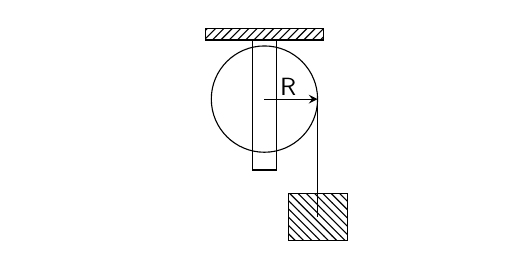
\begin{tikzpicture}[scale=1.5]
\draw[white](-2,0)--(2,0);
\draw[pattern=north east lines] (-0.5,0) rectangle (0.5,0.1);
\draw(0,-0.5) circle (0.45);
\draw[](-0.1,-1.1) rectangle (0.1,0);
\draw[-](0.45,-0.5)--+(0,-1.);
\draw [pattern=north west lines](0.2,-1.3)rectangle(0.7,-1.7);
\draw[-stealth](0,-0.5)--+(0.45,0);
\node at (0.2,-0.4)[scale=0.9]{R};
\end{tikzpicture}
&\\ \hline

7 &
Sebuah bola pejal mempunyai massa $m$ dan jari-jari $r$ menggelinding dari ketinggian 14 cm, berapa kecepatan benda saat mencapai dasar?
& \\ \hline

8 & 

Sebuahtikan gambar berikut! 

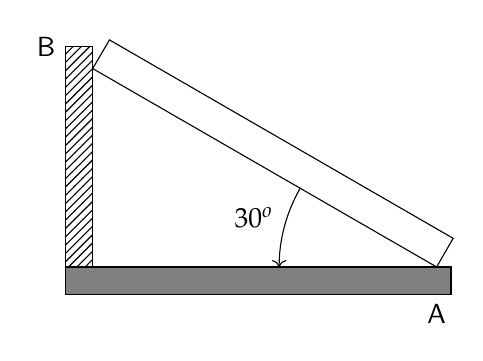
\begin{tikzpicture}[scale=0.7]
\draw(6.24,0)--(0,3.6)coordinate(b);
\draw(6.24,0)--($(6.24,0)+(60:0.6)$)--++(150:7.2)--(b);
\draw [pattern=north east lines] (-0.50,0) rectangle(0,4) ;
\node at (6.24,-0.5)[below]{A};
\node at (-0.5,4)[left] {B};
\coordinate (o) at (0,0);
\coordinate (t) at (6.24,0);
\coordinate (b) at (0,3.6);
    \pic [draw, ->,"$30^o$",angle radius=2cm,  angle eccentricity=1.2] {angle =b--t--o };

\draw [thin, fill =gray] (-0.5,0) rectangle (6.5,-0.5);
\end{tikzpicture}

Diketahui panjang batang AB 2,5 m dan berat 200 N serta batang bersandar pada dinding yang licin. Bila sistem batang dalam keadaan setimbang, maka koefisien gesekan batang dengan lantai adalah . . .  
& \\ \hline

9 &

& \\ \hline

\end{longtable}
\end{center}
\end{document}

